\providecommand{\main}{../../..}
\documentclass[\main/main.tex]{subfiles}
\begin{document}

\subsection{Esercizio 3}
Si consideri il problema:

\begin{align*}
  \max f_1 = x_1 + 3x_2  \\
  \max f_2 = -3x_1 -2x_2 \\
  2x_1 + x_2 & \leq 32   \\
  x_1 + x_2  & \leq 20   \\
  x_1 + 5x_2 & \leq 72   \\
  x_1, x_2   & \geq 0    \\
\end{align*}

Usando curve di indifferenza del tipo $u (f_1, f_2) = 2f_1 + f_2$, si determini la soluzione ottima.

\subsection{Risoluzione esercizio 3}

\subsubsection*{Costruisco funzione di ottimo}

\[
  u (f_1, f_2) = 2\rnd{x_1 + 3x_2} + -3x_1 - 2x_2 = -x_1 + 4x_2
\]

\subsubsection*{Costruisco problema PL}

\begin{align*}
  \max u = -x_1 + 4x_2 \\
  2x_1 + x_2 & \leq 32 \\
  x_1 + x_2  & \leq 20 \\
  x_1 + 5x_2 & \leq 72 \\
  x_1, x_2   & \geq 0  \\
\end{align*}

La soluzione ottima si trova in $O = (0, \frac{72}{5})$

\subsubsection*{Verifico soluzione}

\begin{figure}
  \begin{subfigure}{0.45\textwidth}
    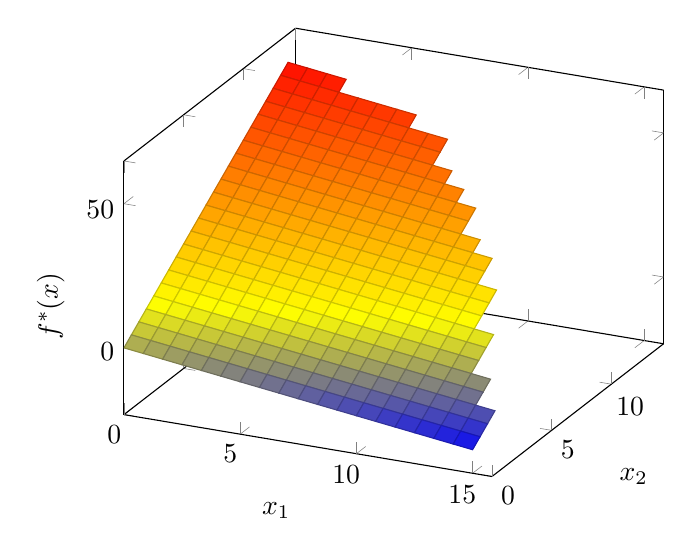
\begin{tikzpicture}
      \begin{axis}[
          xlabel=$x_1$,
          ylabel=$x_2$,
          zlabel=$f^*(x)$,
          domain=0:20,
          y domain=0:15
        ]
        \addplot3[surf, unbounded coords=jump]
        {2*x+y<=32 && x+y <= 20 && x+5*y<=72 ? 4*y-x : NaN};
      \end{axis}
    \end{tikzpicture}
    \caption{La funzione $f^*(x)$}
  \end{subfigure}
  ~
  \begin{subfigure}{0.45\textwidth}
    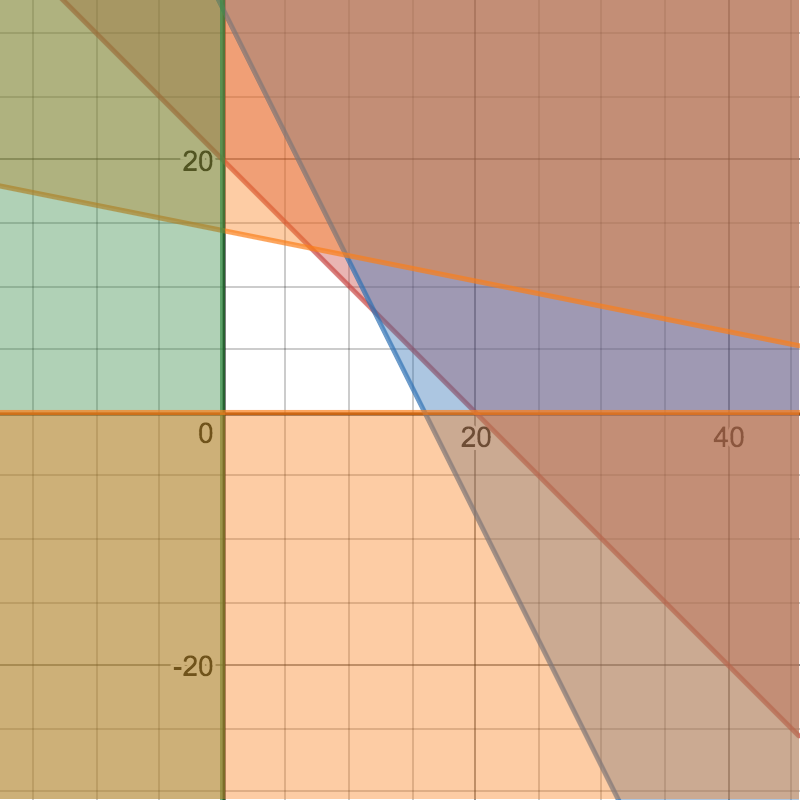
\includegraphics[width=0.8\textwidth]{es3-maut}
    \caption{Dominio della funzione $f^*(x)$}
  \end{subfigure}
\end{figure}

\end{document}